\section{Approach}
    \label{sec:1}
\subsection{Architecture of the model}
The approach chosen for this problem is based on the training of a CNN. The choice of a CNN was clear, as it is a standard model used in computer vision applications. The architecture of the model was determined by trying out different approaches on the raw data to get a feeling for what works and what should be dismissed. This "trying out" showed, that a high amount of convolutional layers would be needed for the model to work properly. With the amount of data being high, a relatively complex architecture was then chosen for this task, which can be seen in
\autoref{fig:arch}.
\begin{figure}[H]
    \centering
    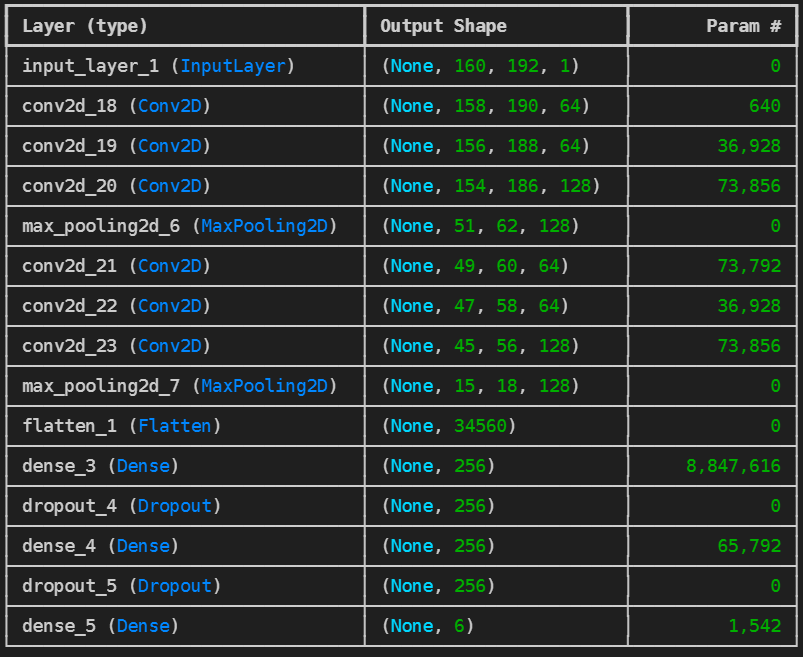
\includegraphics[width=0.7\textwidth]{content/arch.png}
    \caption{Final architecture of the model.}
    \label{fig:arch}
\end{figure}
\noindent
The model consists of two convolutional blocks consisting of 3 convolutional layers and one max-pooling layer respectively. The output of these convolutional blocks is flattened and runs through 2 dense blocks with each one dense layer and one dropout layer.
The number of filters in each block is 64 for the first two convolutional layers and 128 for the last convolutional layer. The kernel size is (3,3) as well as the pool size. 
\subsection{Data preprocessing}
The preprocessing of the data is a crucial step for the success of the chosen method. With the .jpg images being of size (360, 640) and the amount of data being high, down-scaling of the images resolution and size becomes necessary for computation reasons. With this in mind, two methods were implemented, one doing a crop on the image to reduce background, and the other reducing the resolution of the image. 
The initial idea for the cropping was to use a face detection software to dynamically crop each picture according to the drivers face postition. This idea had to be dismissed as the face detection was not as reliable as initially hoped. With many drivers in the "Distraced" class looking to the side or down on their phone, the face detection algorithm started to detect faces in the background of the images, introducing a large bias into the dataset. 
An alternative method was then chosen, which crops 100 pixels from the left and right of every picture, significantly reducing the amount of background for the training of the CNN. A before and after comparison of the cropped images can be seen in \autoref{fig:comp1}
\begin{figure}[H]
    \centering
    \begin{subfigure}{0.48\textwidth}
        \centering
        \adjustbox{valign=c}{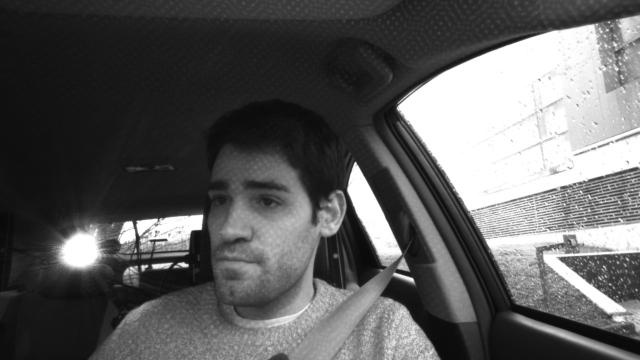
\includegraphics[width = \textwidth]{content/test1.jpg}}
    \end{subfigure}
    \hfill
    \begin{subfigure}{0.48\textwidth}
        \centering
        \adjustbox{valign=c}{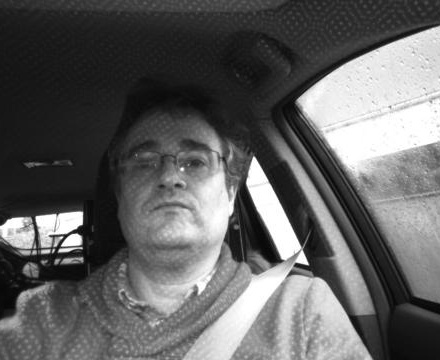
\includegraphics[width = \textwidth]{content/test2.jpg}}
    \end{subfigure}
    \caption{Comparison of the uncropped (left) and cropped (right) images.}
    \label{fig:comp1}
\end{figure}
\noindent
This is possible due to the camera position being relatively consistent throughout all images. A greater crop sometimes led to the faces or class relevant objects being cropped off and was thus not implemented. 
The cropped images were then scaled down to a resolution of 120 $\times$ 100 using the OpenCV \cite{opencv} library.
\section{Data augmentation and overfitting optimization}
    \label{sec:2}
This section will present the precautions taken to compensate for possible overfitting of the data and the data augmentation done to balance the amount of classes in the dataset.
\subsection{Data augmentation}
Classes like "Yawn" or "Drinking" have very few entry in contrast to the rest of the dataset, with relative amounts to the total dataset size being 
Safe driving: $41.59\%$,
Dangerous driving: $31.25\%$,
Distraced: $14.00\%$,
Sleepy driving: $6.59\%$,
Yawn: $3.68\%$,
Drinking: $2.89\%$ .
For this reason data augmentation is implemented to account for the drastic class imbalances.
The original approach for the augmentation process was to generate augmented data to fill up all classes to the number of entries of the largest class. This resulted in an immense amount of data being generated which could not be handled by the computational power avaiable. An alternative approach was then chosen, in which all classes are scaled to 2000 entries. This resulted in cutting off entries from the top three largest classes and only a minimal amount of data augmentation in the three smallest classes. 
The augmentation was conducted using the tensorflow.keras.preprocessing.image.ImageDataGenerator method, alongside a self implemented noise generator. The ImageDataGenerator does a random augmentation for each image based on initially set parameters. The augmentations applied to the images are shifts in width and height up to a value of 0.1, shear and zoom up to a value of 0.3 and 0.1 respectively and a possible vertical flip of the image. The noise generator applies random gaussian noise to each pixel, with the strength of the noise being random for each image. A total of 4047 augmented images were generated this way, while 6902 images were cut from the largest classes. 
\begin{figure}[H]
    \centering
    \begin{subfigure}{0.48\textwidth}
        \centering
        \adjustbox{valign=c}{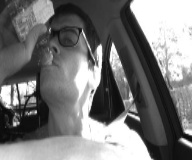
\includegraphics[width = \textwidth]{content/test_aug_1.jpg}}
    \end{subfigure}
    \hfill
    \begin{subfigure}{0.48\textwidth}
        \centering
        \adjustbox{valign=c}{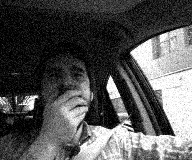
\includegraphics[width = \textwidth]{content/test_aug_2.jpg}}
    \end{subfigure}
    \caption{Two exemplary augmnted pictures with zoom and shear (left) and noise (right).}
    \label{fig:comp2}
\end{figure}
\noindent
Two exemplary augmented pictures can be seen in \autoref{fig:comp2}. The final CNN with optimized hyperparameters was then trained on both the original dataset and the augmented dataset with 2000 entries in each class. While the performance was roughly equal, the confusion matrices show the necessity of equally sized classes.
The confusion matrices for the training on both datasets can be seen in \autoref{fig:comp3}. The matrices' entries have been normalized for the number of entries of each class in the test data respectively, thus showing the recall of the class on the diagonal.
\begin{figure}[H]
    \centering
    \begin{subfigure}{0.49\textwidth}
        \centering
        \adjustbox{valign=c}{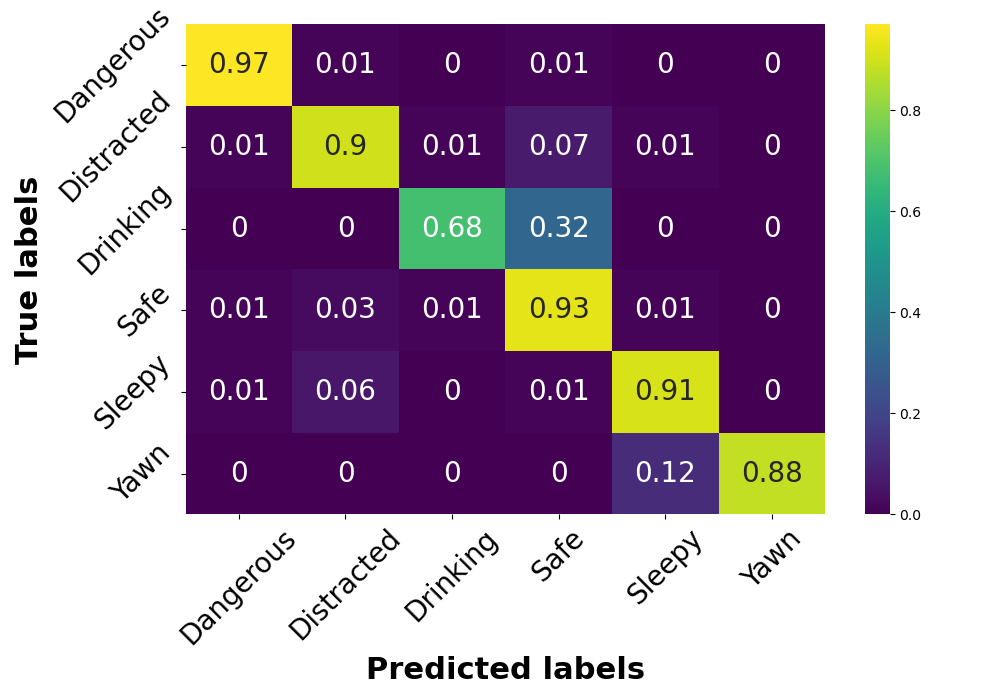
\includegraphics[width = \textwidth]{content/confusion_matrix_final_og_norm.png}}
        \caption{Original dataset.}
    \end{subfigure}
    \hfill
    \begin{subfigure}{0.49\textwidth}
        \centering
        \adjustbox{valign=c}{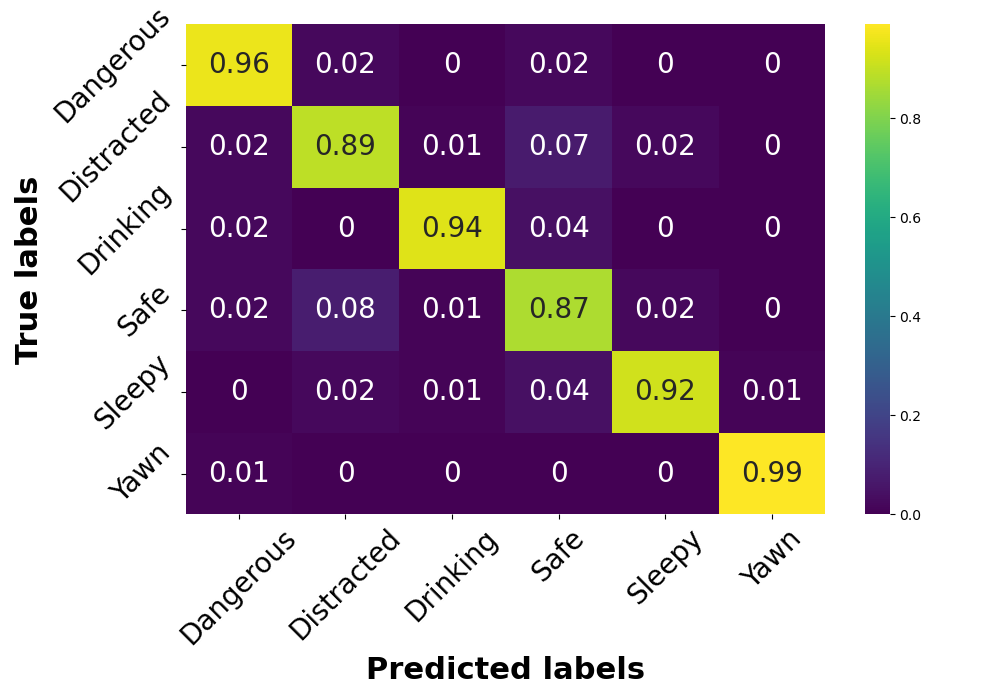
\includegraphics[width = \textwidth]{content/confusion_matrix_final_aug_norm.png}}
        \caption{Augmented dataset.}
    \end{subfigure}
    \caption{Confusion Matrices on the test data of the original dataset (left) and the augmented dataset (right).}
    \label{fig:comp3}
\end{figure}
\noindent
The left confusion matrix of the original dataset shows huge amounts of miss classification of pictures labeled "Drinking". This is not only due to an inacurate prediction, but also due to the small amount of entries labeled "Drinking" in the original test data, with a total of only 25 "Drinking" images. This shows a signigicantly decreased sensitivity in the low number of entries classes in comparison to the confusion matrix of the augmented dataset. For these reasons the augmented dataset was chosen for the final comparison to the alternative model, showing a good recall in all of its classes.
\subsection{Overfitting optimization}
To avoid overfitting, several methods were implemented. The model itself contains 2 dropout layers with one in each dense block. These layers reduce overfitting as dropping out neurons during the training process is a form of regularization. Further regularization is introduced into the model by applying a L2 regularization to the loss function. This regularization penalizes large weights, leading to a reduction of the models complexity, which can be a reason for bad performance on unseen data. Both the dropout rate and regularization strength are hyperparameters, whose optimal values are obtained in the hyperparameter optimization. This leads to these methods being nearly optimally tuned to reduce overfitting.
\begin{figure}[H]
    \centering
    \begin{subfigure}{0.49\textwidth}
        \centering
        \adjustbox{valign=c}{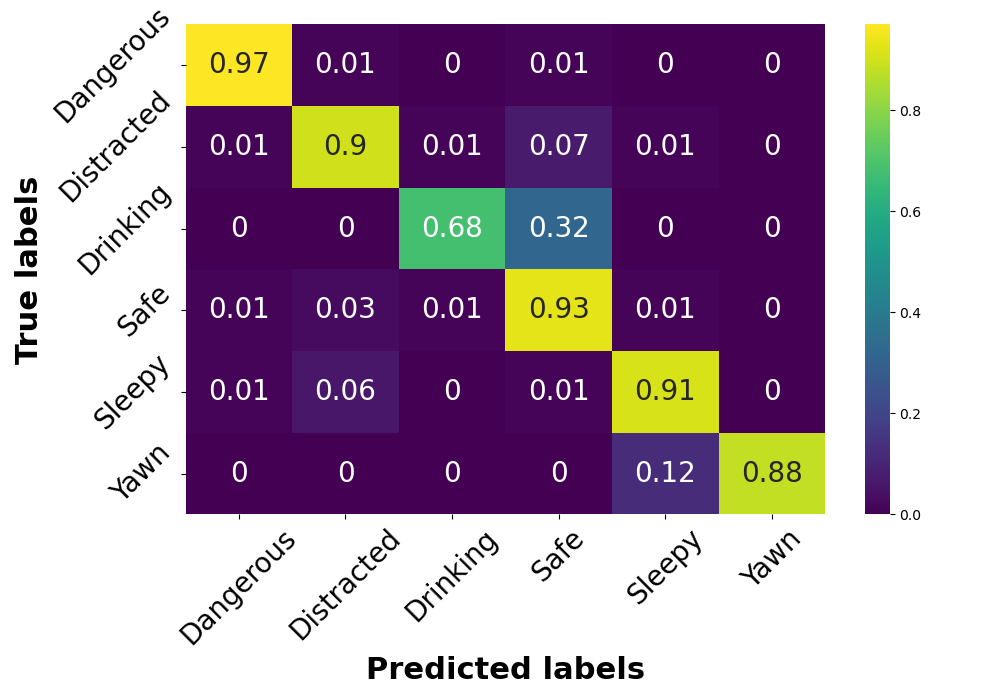
\includegraphics[width = \textwidth]{content/confusion_matrix_final_og_norm.png}}
        \caption{loss before hyperparameter opt.}
    \end{subfigure}
    \hfill
    \begin{subfigure}{0.49\textwidth}
        \centering
        \adjustbox{valign=c}{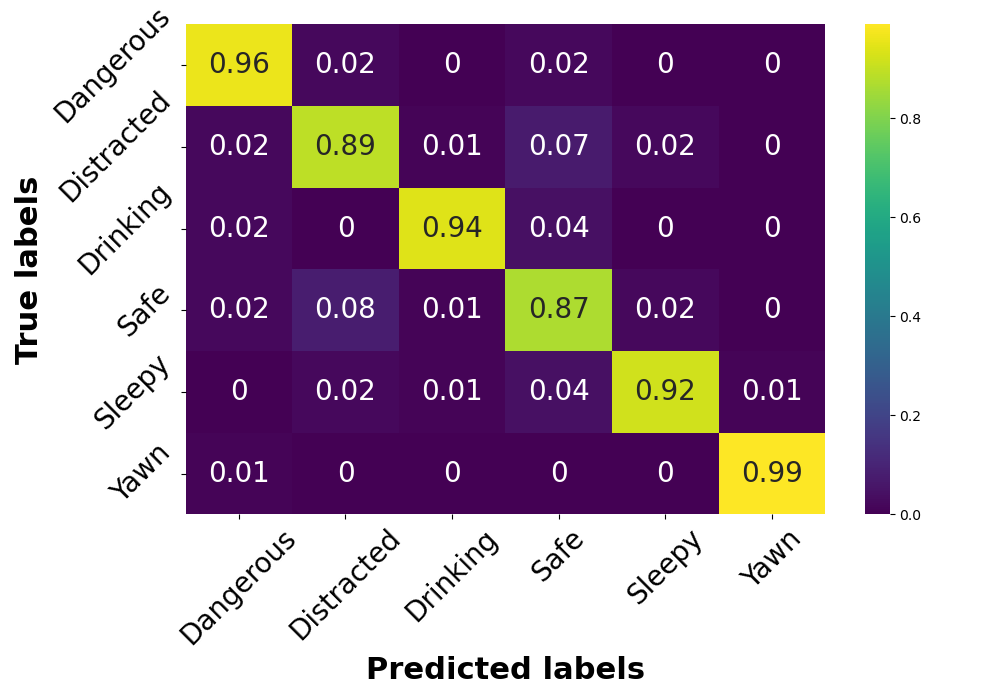
\includegraphics[width = \textwidth]{content/confusion_matrix_final_aug_norm.png}}
        \caption{loss before hyperparameter opt.}
    \end{subfigure}
    \caption{placeholde.}
    \label{fig:comp3}
\end{figure}
\noindent
(ref) shows the loss per epoch before and after the hyperparameter optimization. Without optimized parameters in these regularization methods, the loss on the left shows clear signs of overfitting. While the optimized loss on the right shows a much better result, it still runs into overfitting after a greater amount of epochs. This is due to the limited size of the augmented dataset chosen, with a larger dataset having too much computational cost. A larger dataset would not run into overfitting as fast, but resulted in crashes on the used hardware. To combat this phenomenon early stopping was implemented, which set the CNN's weights to the optimal values of a previous epoch once a stagnation in the validation loss is detected. This prevents the usage of an overfit model even though the training eventually runs into overfitting.
To further ensure the validity of the obtained results against the chosen alternative method. All obtained results in the next chapter are cross validated in a six-fold cross validation. This ensures a generalized validity of the presented results and combats overfitting as the used training data is varies for each combination of folds.
\section{Results and comparison to alternative Method}
    \label{sec:3}